% docx2tex --- ``Garbage In, Garbage Out''
%
% docx2tex is Open Source and
% you can download it on GitHub:
% https://github.com/transpect/docx2tex
%
\documentclass{article}
\usepackage{graphicx}
\usepackage{hyperref}
\usepackage{multirow}
\usepackage{tabularx}
\usepackage{color}
\usepackage{amsmath}
\usepackage{amssymb}
\usepackage{amsfonts}
\usepackage{amsxtra}
\usepackage{wasysym}
\usepackage{isomath}
\usepackage{mathtools}
\usepackage{txfonts}
\usepackage{upgreek}
\usepackage{enumerate}
\usepackage{tensor}
\usepackage{pifont}
\usepackage{float}
\usepackage{fancyhdr}
\usepackage{lastpage}
\usepackage{incgraph}
\usepackage{changes}
\usepackage{pdfpages}
\usepackage{xr}
\externaldocument[R-]{rules}


\usepackage[letterpaper, margin=1in, headheight=47pt]{geometry}

% No paragraph indent
\setlength{\parindent}{0cm}
% Bigger paragraph skips
\setlength{\parskip}{0.25cm}

% TEX Gyre Adventor font (looks pretty nice)
\renewcommand*\rmdefault{qag}

\pagestyle{fancy}

\lhead{}
\chead{}
\rhead{
\includegraphics[width=8cm]{media/image15.png}}
\renewcommand{\headrulewidth}{0pt}
%\renewcommand{\topmargin}{-20pt}

\rfoot{Page \textbf{\thepage} of \textbf{\pageref{LastPage}}}
\lfoot{\textit{Draft as of \today}}
\cfoot{}

% First page
\fancypagestyle{firststyle}{%
  \fancyhf{}
  \fancyfoot[L]{\textit{Draft as of \today}}
  \fancyfoot[R]{Page \textbf{\thepage} of \textbf{\pageref{LastPage}}}
}

\definechangesauthor[color=red]{TC}
\setdeletedmarkup{\footnote{In previous version of the rules this was ''\emph{#1}''}}
\setauthormarkup{}

\title{\vspace{-5ex}RoboCupJunior Soccer Super Team Rules 2018\vspace{-5ex}}
\date{\vspace{-2ex}}
%\date{Draft as of \today}

\definecolor{color-1}{rgb}{1,1,1}
\definecolor{color-2}{rgb}{0,0,0.5}
\definecolor{color-3}{rgb}{0.07,0.33,0.8}
\definecolor{color-4}{rgb}{0.13,0.13,0.13}
\definecolor{red}{rgb}{1,0,0}
\definecolor{color-6}{rgb}{0,0,1}



\begin{document}
\maketitle
\thispagestyle{firststyle}

\textbf{Soccer Technical Committee 2018:}

\resizebox{0.45\textwidth}{!}{
\begin{tabular}{lr}
    Sarit Salzman             & Israel\\
    James Riley               & Australia\\
    Javier E. Delgado Moreno  & Mexico \\
    Michael Sloan Warren      & USA\\
    Felipe Nascimento Martins & Netherlands\\
    Marek \v{S}uppa           & Slovakia (CHAIR)\\
\end{tabular}}

These are the official Soccer rules for RoboCupJunior 2018. They are released
by the RoboCupJunior Soccer Technical Committee. The English version of these
rules has priority over any translations. \textcolor{red}{\textbf{Items in red
represent significant rules changes introduced this year.}}

Teams are advised to check the RoboCupJunior Soccer site
\href{http://rcj.robocup.org/soccer.html}{http://rcj.robocup.org/soccer.html}
for OC (Organizational Committee) procedures and requirements for the
international competition. Each team is responsible for verifying the latest version of the
rules prior to competition.

\section*{Preface}

In the RoboCupJunior soccer challenge, teams of young engineers design, build,
and program two fully autonomous mobile robots to compete against another team
in matches. The robots must detect a ball and score into a color-coded goal on
a special field that resembles a human soccer field.

To be successful, participants must demonstrate skill in programming, robotics,
electronics and mechatronics.  Teams are also expected to contribute to the
advancement of the community as a whole by sharing their discoveries with other
participants and by engaging in good sportsmanship,regardless of culture, age or
result in the competition. \textbf{All are expected to compete,
learn, have fun, and grow.}


These rules are released together with the current regular game rules. Wherever
a change is needed because of the difference with regular games, situation have
been analyzed and are ruled here. For all other situations that do not change
from the regular game rules, normally they have been only mentioned here as
being the same regular game rule.

\listofchanges
\newpage

\tableofcontents

\newpage

\section{GAMEPLAY \label{ref-001}}

\subsection{Game procedure and length of a game \label{ref-002}}

The game will consist of two halves. The duration of each half is 10-minutes.
There will be a 5-minute break in between the halves.

The game clock will run for the duration of the halves without stopping (except
if or when a referee wants to consult another official). The game clock will be run
by a referee or a referee assistant (see Rule 7.1 for the description of a
referee assistant).


SuperTeam are supposed to be at their big field 10 minutes before their game
starts. To be at the inspection table does not count in favor of this time
limit.

\replaced[id=TC]{SuperTeams that are late for the start of the game can be penalized
one goal per 30 seconds at the referee's discretion. In this (and any)
situation, when the goal differential reaches 10 the game finishes regardless
of the state of the game clock.}{SuperTeams can be penalized one goal per each
elapsed 30 seconds at the referee's discretion if they are late for the game
start. In any situation, when the goal difference reaches 10, the game finishes
regardless of the state of the game clock.}

\subsection{Pre-match meeting \label{ref-003}}

At the start of the first half of the game, a referee will toss a coin. The
SuperTeam mentioned first in the draw shall call the coin. The winner of the toss
can choose either which end to kick towards, or to kick off first. The loser of the
toss chooses the other option. After the first half, SuperTeams switch sides.
The SuperTeam not kicking off in the first half of the game will kick off to
begin the second half of the game.

\added[id=TC]{During the pre-match meeting the referee or their assistant may
check whether the robots are capable of playing (i.e., whether they are at
least able to follow and react to the ball). If none of the robots (of any
team) is capable of playing, the game will not be played and zero goals will
be awarded to both teams.}

\subsection{Kick-off \label{ref-004}}

Each half of the game begins with a kick-off. All robots must be located on
their own side of the field. All robots must be halted. The ball is positioned
by a referee in the center of the field.

Each SuperTeam has to position one robot as a goalie (fully inside their
penalty area), and the rest of the robots can be located anywhere on their side
of the playing field, as long as they are at a maximum distance of 10 cm from
any white line.

The SuperTeam kicking off places their robots on the big field first. Robots
cannot be repositioned once they have been placed.

The SuperTeam not kicking off will now place their robots on the defensive end
of the big field.

A referee may adjust the placement of the robots to make sure that the robots
are placed properly within the big field positions.

\added[id=TC]{Robots cannot be placed behind the goal line or out of bounds.
Robots cannot be repositioned once they have been placed, except if the referee
requests to adjust their placement to make sure that the robots are placed
properly within the field positions.}

On the referee's command (usually by whistle), all robots will be started
immediately by each captain. Any robots that are started early will be removed
by the referee from the field and treated as a damaged robot.

\subsection{Human interference\label{ref-005}}

Except for the kick-off, human interference from SuperTeam members (e.g.
touching the robots) during the game is not allowed unless explicitly permitted
by a referee. Violating SuperTeam / SuperTeam member(s) can be disqualified from
the game.

The referee or a referee assistant can help robots get unstuck if the ball
is not being disputed near them and if the situation was created from normal
interaction between robots (i.e. it was not a design or programming flaw of
the robot alone). The referee or a referee assistant will pull back the robots
just enough for them to be able to move freely again.

\subsection{Ball movement \label{ref-006}}

RoboCupJunior Soccer Rules 2018 rule \ref{R-ref-ball-movement} applies.

\subsection{Scoring \label{ref-007}}

A goal is scored when the ball strikes or touches the back wall of the goal.
Goals scored either by an attacking or defending robot have the same end
result: they give one goal to the SuperTeam on the opposite side. After a goal,
game will be restarted with a kick-off from the SuperTeam who received the goal
against. After the referee signals that a goal was scored, the referee will
invite SuperTeam members to capture their robots or ask a referee to help
capture them and get ready for kick-off. Before a kick-off, all damaged or
out-of-bounds robots are allowed to return to the playing field immediately if
they are ready and fully functional.

\subsection{Goalie \label{ref-008}}

The robot moving first into the penalty area on a SuperTeam's defending side
completely (with every part of it) is designated as goalie until a part of it
leaves the penalty area.

\subsection{Pushing \label{ref-009}}

RoboCupJunior Soccer Rules 2018 rule \ref{R-ref-pushing} applies.

\subsection{Lack of progress \label{ref-010}}

RoboCupJunior Soccer Rules 2018 rule \ref{R-ref-lack-of-progress} applies.

\subsection{Out of bounds \label{ref-011}}

If a robot's entire body moves out beyond the white line of the big field
completely, it will be called for being out of bounds. When this situation
arises, the robot is given a one-minute penalty, and the SuperTeam is asked to
remove the robot from the big field. There is no time stoppage for the game
itself. The robot is allowed to return if a kickoff occurs before the penalty
has elapsed.

The one-minute penalty starts when the robot is removed from play. Furthermore,
any goal scored by the penalized team while the penalized robot is on the field
will not be granted. Out-of-bounds robots can be fixed if the SuperTeam needs
to do so, as described in 1.11.

After the penalty time has passed, robot will be placed on the unoccupied
neutral spot nearest to where it has been taken off, \replaced[id=TC]{and not
directly aiming towards the ball}{orientated towards the nearest wall}.
\added[id=TC]{Alternatively, the referee may instruct the
team to place the robot on the neutral spot on the side of the field
currently farthest from the ball, oriented towards the closest wall. }

A referee can waive the penalty if the robot was accidentally pushed out of
bounds by \replaced[id=TC]{an opposing}{any other} robot. In such a case, the
referee may have to slightly push the robot back onto the field.

The ball can leave and bounce back into the playing field. The referee calls
``out of reach'', and will move the ball to the nearest unoccupied neutral spot
when one of the following condition occurs:

\begin{enumerate}
    \item the ball remains outside the playing field too long,
        after a visible and loud count, (usually a count of five, the length of
        the count can be decided by the OC before a competition as long as it
        is the same length within a sub-league)

    \item any of the robots are unable to return it into the playing field
        (without their whole body leaving the playing field), or

    \item the referee determines that the ball will not come back into the
        playing field.

\end{enumerate}

\subsection{Damaged robots \label{ref-012}}

If a robot is damaged, it has to be taken off the field and must be fixed
before it can play again. Even if repaired, the robot must remain off the field
for at least one minute or until the next kickoff is due. If SuperTeam members
cannot reach the damaged robot by themselves without stepping inside the field,
they should ask a referee to hand over the damaged robot.  If all robots have
moved out of bounds, the penalties are discarded and the match resumes with a
neutral kickoff.

Some examples of a damaged robot include:

\begin{itemize}

\item it does not respond to the ball, or is unable to move (it lost pieces,
    power, etc.).

\item it continually moves into the goal or out of the playing field.

\item it turns over on its own accord.

\end{itemize}


Computers and repair equipment are not permitted in the playing area during
gameplay. Usually, a SuperTeam member will need to take the damaged robot to an
``approved repair table'' near the playing area.\deleted[id=TC]{, located
inside the competitors working area.} A referee may permit robot sensor
calibration, computers and other tools in the playing area, only for the 5
minutes before the start of each half. \added[id=TC]{Reprogramming of robots
during the gameplay can only happen when they are out of game (i.e., damaged
or out of bounds), or when explicitly allowed by the referee.}

After a robot has been fixed, it will be placed on the unoccupied neutral spot
nearest to where it has been taken off, \replaced[id=TC]{and not directly aiming
towards the ball}{orientated towards the nearest wall}.
\added[id=TC]{Alternatively, the referee may instruct the team to place
the robot on the neutral spot on the side of the field currently farthest from
the ball, orientated towards the nearest wall.}
A robot can only be returned to the field if the damage has been
repaired. If the referee notices that the robot was returned to the field with
the same original problem, s/he may ask the robot to be removed, and proceed
with the game as if the robot had not been returned.

\textbf{Only the referee decides whether a robot is damaged.} A robot can only
be taken off or returned with the referee's permission.

\replaced[id=TC]
{
If all robots from the same SuperTeam are deemed damaged at kickoff,
gameplay will be paused and the remaining team will be awarded 1 goal for
every 30 seconds that their opponent's robots remain damaged.
}
{
If all robots from the same SuperTeam are deemed damaged during gameplay, the
clock continues and the remaining SuperTeam gets one initial goal and rests
while waiting for the opponent's return to play. The remaining SuperTeam will
also get one additional goal for each minute the opponent's robots remain
damaged. After five minutes of absence, the SuperTeam with no functional robots
forfeits the game.
}

However, these rules only apply when none of the two robots from the same team
were damaged as the result of the opponent team violating the rules.

\subsection{Multiple defense \label{ref-013}}

Multiple defense occurs if more than one robot from the defending SuperTeam
enters its penalty area with some part and substantially affects the game.
\replaced[id=TC]{All robots except for the one closest to}{The robot farther
from} the ball will be moved to the nearest corner. The referee could take this
action at any time when more than one robot lingers in their penalty area.

\added[id=TC]{Only} the referee can take this action at any time when both
robots linger in their penalty area.

\added[id=TC]{If multiple defense happens repeatedly in a short amount of time,
the offending robot will be moved to an unoccupied neutral spot on the other
side of the field, orientated towards the nearest wall.}
\replaced[id=TC]{If any robot needs to be moved to an unoccupied neutral spot
more than \textbf{three times} during its single uninterrupted time chunk on the
field, it}{If multiple defense happens repeatedly, the robot}
will be deemed damaged\footnote{For the purpose of this rule a time chunk is
defined as time between two events when the robot is taken off the field for
some reason (e.g. at the end of the first half of the game, when it is deemed
damaged or out of bounds).}.

\subsection{Interruption of Game \label{ref-014}}

RoboCupJunior Soccer Rules 2018 rule \ref{R-ref-interruption} applies.

\section{SUPERTEAM \label{ref-015}}

\subsection{Regulations \label{ref-016}}

A SuperTeam is a team of 3 or more regular teams with their corresponding
robots, all from the same sub-league. Regular team is defined on RoboCupJunior
Soccer Rules 2018 rules \ref{R-ref-team-regulations} and
\ref{R-ref-number-of-robots}. Each regular team is required to provide at least
one robot for each SuperTeam game.

Each SuperTeam must have a captain. The captain is the person responsible for
communication with referees. The SuperTeam can replace its captain during
gameplay. SuperTeam is allowed to have only the fewest possible members beside
the field during game play: they will usually be the captain and one member
from each individual team who has a robot as an active SuperTeam player (see
Soccer Rules 2018 rule \ref{R-ref-team-regulations}).

\subsection{Violations \label{ref-017}}

RoboCupJunior Soccer Rules 2018 rule \ref{R-ref-violations} applies.

\section{ROBOTS\label{ref-018}}

\subsection{ Number of robots / substitution \label{ref-019}}


The SuperTeam will have all the robots from their respective individual teams
available to play. In the playing field, the SuperTeam is allowed to use a
maximum of 5 robots simultaneously, and they are its active players. The rest
of the robots constitute their reserve players. Since the playing field is big,
it is suggested that the SuperTeam establish positions for the robots inside
the playing field (goalkeeper, backs, midfielders, forwards, etc.), by
adjusting robot's mechanics and programming.


The substitution of robots during the competition with other SuperTeam is
forbidden. Robots will be issued a special code that will distinguish them from
other SuperTeams. Each robot that belongs to a superteam will receive an ID
identifying the robot as being a member of a team.

Example: Robot A-2: the referee would identify robot with sticker A-2 as robot
number 2 belonging to team A. These IDs will be written on the Top Markers of
robots (see RoboCupJunior Soccer Rules 2018 rule \ref{R-ref-top-markers}).


Each individual team is required to have at least one of its robots as an
active player, with the exception of a sixth team in which case SuperTeam is
required to have individual team rotation allowing with that to include all
individual teams evenly. SuperTeam members can decide freely how to substitute
robots between the current players and the reserve players during gameplay, but
the captain is required to ask a referee for robot substitution authorization.
Substitutions are allowed only at every kick-off (see rule 5.3).

\subsection{ Interference \label{ref-020}}


RoboCupJunior Soccer Rules 2018 rule \ref{R-ref-interference} applies.


\subsection{ Control \label{ref-021}}

RoboCupJunior Soccer Rules 2018 rule \ref{R-ref-control} applies.

\subsection{ Communication \label{ref-022}}

Robots are not allowed to use any kind of communication during game play unless
the communication between two robots is via Bluetooth class 2 or class
3\footnote{range shorter than 20 meters} or via any other device that
communicates using the 802.15.4 protocol (e.g., ZigBee and XBee). SuperTeams
are responsible for their communication. The availability of frequencies cannot
be guaranteed.

\subsection{Agility \label{ref-023}}


RoboCupJunior Soccer Rules 2018 rule \ref{R-ref-agility} applies.


\subsection{ Handle \label{ref-024}}


RoboCupJunior Soccer Rules 2018 rule \ref{R-ref-handle} applies.

\subsection{ Top Markers\label{ref-025}}


RoboCupJunior Soccer Rules 2018 rule \ref{R-ref-top-markers} applies.


\subsection{ Additional regulations of the sub-leagues \label{ref-026}}

RoboCupJunior Soccer Rules 2018 rule \ref{R-ref-sub-leagues} applies.

\subsection{ Violations \label{ref-027}}

Robots that do not abide by the specifications/regulations are not allowed to
play. If violations are detected during a running game, the SuperTeam is
disqualified for that game. If similar violations occur repeatedly, the
SuperTeam can be disqualified from the tournament.

\section{BIGFIELD \label{ref-028}}

\subsection{Kind of field \label{ref-029}}

There is only one kind of field for all sub-leagues.

\subsection{ Dimensions of the field \label{ref-030}}

The big field is 540 cm by 340 cm. The big field is marked by a white line that
is part of the playing field. Around the playing field, beyond the white line,
is an outer area of 30 cm width. Total dimensions of the big field, including
the outer area, are 600 cm by 400 cm. The playing area is divided in sides for
each SuperTeam by a black line. The field is located 70 cm above the floor.

\subsection{ Walls \label{ref-031}}


Walls are placed all around the big field, including behind the goals and the
out-area. The height of the walls is 22 cm. The walls are painted matte black.
RoboCupJunior Soccer Rules 2017 rule \ref{R-ref-walls} applies with regards to
the landmarks placed on the walls.

\subsection{ Goals \label{ref-032}}


The big field has two goals, centered on each of the shorter sides of the
playing field. The goal inner space is 60 cm width, 10 cm high and 74 mm deep,
box shaped. It has a cross-bar on top (to prevent robots from entering the goal
and to allow checking if the ball scored). The goal ``posts'' are positioned
over the white line marking the limits of the big field. The cross-bar is
exactly over the white line. The height of the cross-bar is 2 cm. The interior
walls and the cross-bar of each goal are painted, one goal yellow, the other
goal blue. The exterior (including the goal post and frame) are painted black.

\subsection{ Floor \label{ref-033}}

The floor consists of green carpet on top of a hard surface.
\deleted[id=TC]{The carpet should be of a quality that will resist the wear and
tear of spinning wheels.} All straight lines on the big field should be painted
and have a width of 20 mm. It is recommended the floor near the exterior wall
to have a wedge, which is an incline of 10 cm base and 2 cm rise for allowing
the ball to roll back into play when it leaves the playing field.

\subsection{ Neutral spots \label{ref-034}}

There are five neutral spots defined in the big field. One is in the center of
the big field. The other four are located over the diagonals that go through
the corners of the playing field, half the distance between the center of the
field and each corner. The neutral spots can be drawn with a thin black marker.
The neutral spots ought to be of circular shape measuring 1 cm in diameter.

\subsection{ Center circle \label{ref-035}}

A center circle will be drawn on the big field. It is 80 cm in diameter. It is
a thin black marker line. It is there for Referees and SuperTeam members as
guidance during kick-off.

\subsection{ Penalty areas \label{ref-036}}

In front of each goal there is a 35 cm wide and 120 cm long penalty area.

The penalty areas are marked by a black line of 20 mm width. The line is part of the area.

A robot is considered inside the Penalty Area when it is completely inside.

\subsection{Lighting and Magnetic Conditions \label{ref-037}}


RoboCupJunior Soccer Rules 2018 rule \ref{R-ref-lighting-conditions} applies.

\section{BALL \label{ref-038}}


RoboCupJunior Soccer Rules 2018 rules \ref{R-ref-sec-spec-plused},
\ref{R-ref-sec-spec-open} and \ref{R-ref-tournament-balls} applies.

\section{CODE OF CONDUCT\label{ref-040}}

All rules in RoboCupJunior Soccer Rules 2018  section
\ref{R-ref-code-of-conduct} apply.

\section{CONFLICT RESOLUTION \label{ref-047}}

All rules in RoboCupJunior Soccer Rules 2018  section
\ref{R-ref-conflict-resolution} apply.

\section*{BIG FIELD DIAGRAM}
\begin{center}
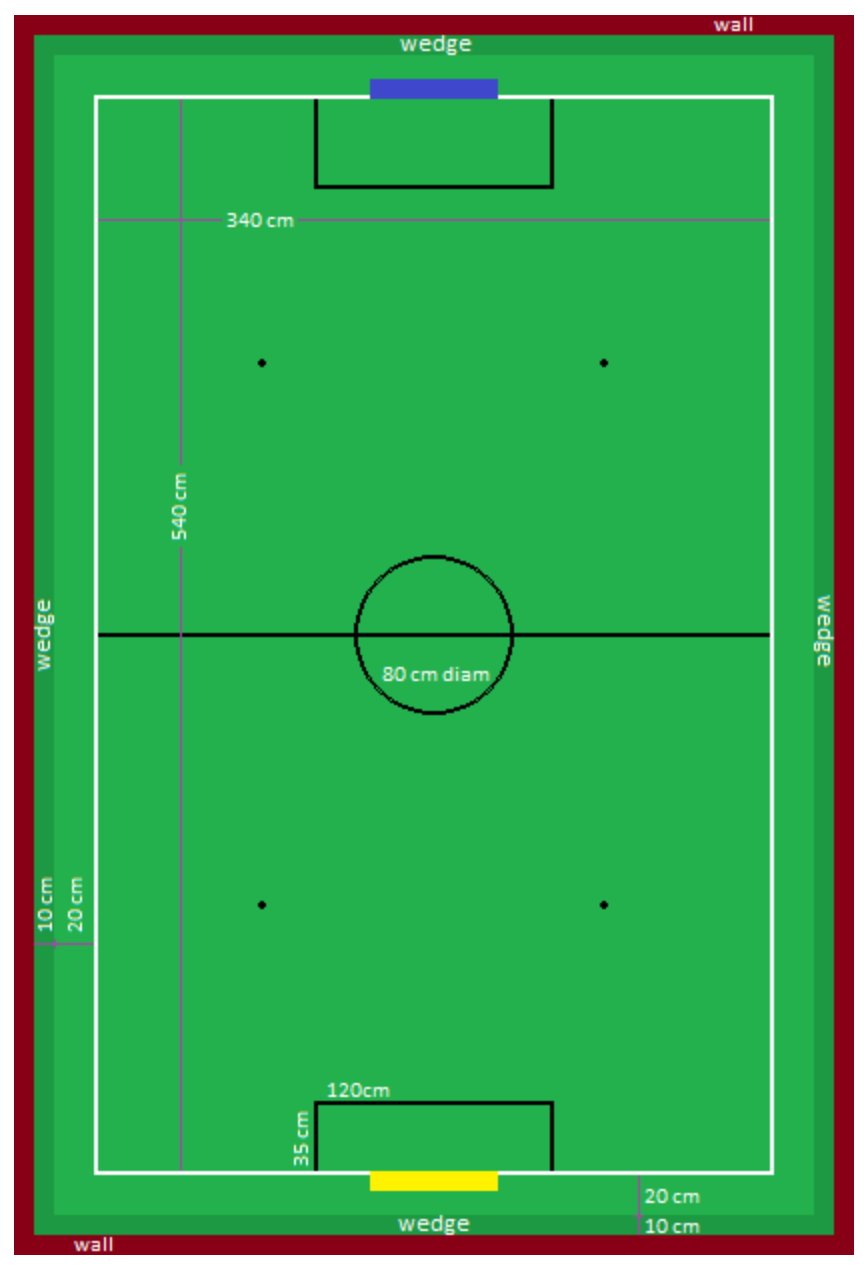
\includegraphics[width=0.9\textwidth]{media/bigfield.png}
\end{center}
\end{document}
